\begin{theo}[Magnetisch veld ten gevolge van een rechte draad]{Magnetisch veld ten gevolge van een rechte draad}
    \begin{minipage}{0.87\textwidth}
        Het magnetische veld ten gevolge van de elektrische stroom in een lange rechte draad is zodanig dat de
        veldlijnen cirkels zijn met de draad in het midden (zie figuur). De veld sterkte is groter hoe dichter je bij de
        draad bent en hoe groter de stroom, in formulevorm:
        \begin{equation*}
            B \propto \dfrac{I}{r}
        \end{equation*}
        met r de loodrechte afstand van de draad. Deze relatie blijft waar als we aanemen dat de draad lang is.
        Het magnetisch veld nabij een lange, rechte draad is als volgt
        \begin{equation*}
            B = \dfrac{\mu_0}{2\pi}\dfrac{I}{r}
        \end{equation*}
        met $\mu_0$ de magnetische permeabiliteit in vacuum.
    \end{minipage}
    \begin{minipage}{.09\textwidth}
        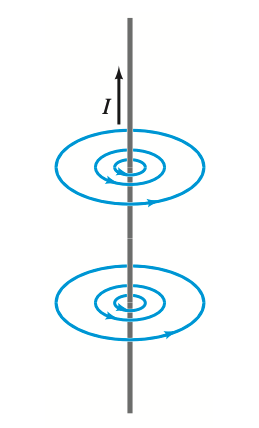
\includegraphics[scale=0.225]{Images/Magnetisme/MagnetischVeldTenGevolgeRechteDraad}
    \end{minipage}
\end{theo}

\begin{app}[Magnetische kracht tussen twee parallelle draden]{Magnetische kracht tussen twee parallelle draden}
    \begin{minipage}{0.77\textwidth}
        Neem twee lange evenwijdige draden gescheiden door een afstand d, zoals in de figuur. Ze voeren respectievelijk stromen $I_1$ en $I_2$.
        Elke stroom produceert een magnetisch veld dat door de ander wordt ‘gevoeld’, dus oefenen ze een kracht uit op mekander.
        We weten dat
        \begin{equation*}
            F_{\parallel} = I\ell B
        \end{equation*}
        en dus krijgen we
        \begin{equation*}
            F = I_{2}B_{1}\ell_{2} = \dfrac{\mu_0}{2\pi}\dfrac{I_{1}I_{2}}{d}\ell_{2}
        \end{equation*}
    \end{minipage}
    \begin{minipage}{.19\textwidth}
        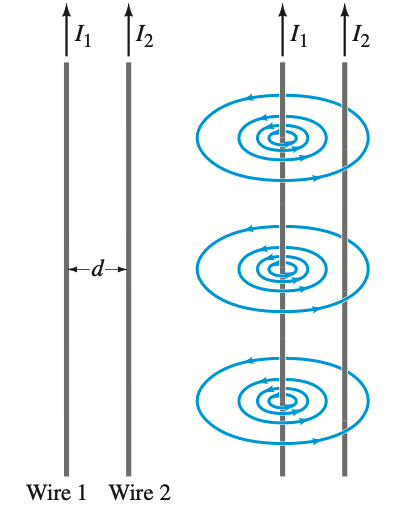
\includegraphics[scale=0.225]{Images/Magnetisme/MagnetischeKrachtTussenTweeParallelleDraden}
    \end{minipage} \vspace{0.2cm}\\
    waarbij we bovenstaande definitie toepassen. Hieruit kunnen we afleiden dat evenwijdige stroomvoerende geleiders elkaar
    \begin{itemize}
        \item aantrekken indien de stroom in dezelfde richting vloeit,
        \item afstoten indien de stroom in tegengestelde richting vloeit.
    \end{itemize}
\end{app}

\begin{lem}[Ampère]{Ampère}
    \vspace{-0.75cm}\begin{minipage}{0.79\textwidth}
        De lijnintegraal van het magneetveld langs een gesloten pad is gelijk aan $\mu_{0}I_{\text{in}}$, waarbij $I_{\text{in}}$ de totale stroom is, die vloeit door een oppervlak dat omsloten is door het pad, in formulevorm:
        \begin{equation*}
            \oint \Vec{B} \cdot d\Vec{\ell} = \mu_{0}I_{\text{in}}
        \end{equation*}
    \end{minipage}
    \begin{minipage}{.17\textwidth}
        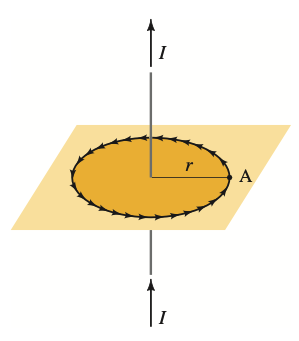
\includegraphics[scale=0.3]{Images/Magnetisme/WetVanAmpere}
    \end{minipage}
\end{lem}

\newpage

\begin{theo}[Magnetisch veld van een spoel]{Magnetisch veld van een spoel}
    Een lange draad met meerdere windingen noemen we een \textbf{spoel}, zie de figuur hieronder.

%    \vspace{0.5cm}

%    \begin{minipage}{.48\textwidth}
        \begin{center}
%            Spoel: \\
            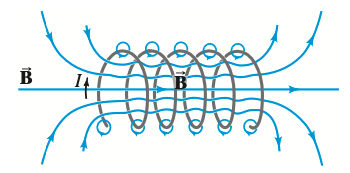
\includegraphics[scale = 0.45]{Images/Magnetisme/Spoel}
        \end{center}
%    \end{minipage}
%    \begin{minipage}{.48\textwidth}
%        \begin{center}
%            \vspace{0.75cm}
%            Dicht gepakte spoel: \\
%            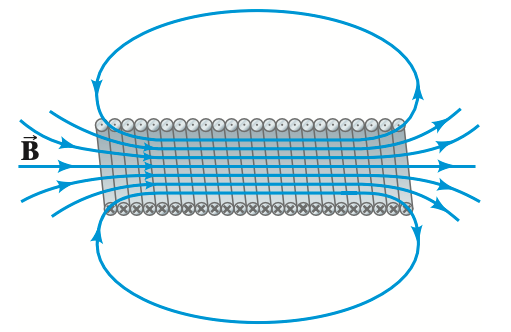
\includegraphics[scale = 0.25]{Images/Magnetisme/SpoelDicht}
%        \end{center}
%    \end{minipage}

%    \vspace{0.5cm}

    \noindent Elke winding genereert een magnetisch veld. Nabij elke draad zijn de veldlijnen quasi cirkels, net zoals bij een rechte draad. 
    In het centrum van de spoel is het netto magnetisch veld een redelijkgroot en redelijk uniform veld, we nemen aan dat een spoel dicht gebonden is en dus dat het veld praltisch uniform is.
    We kunnen de wet van Ampère toepassen op de zijden van de rechthoek (zie figuur onderaan)
    \begin{align*}
       \hspace{1cm}
        \oint \Vec{B} \cdot d\Vec{\ell} &= \int_{a}^{b} \Vec{B} \cdot d\Vec{\ell} + \int_{b}^{c} \Vec{B} \cdot d\Vec{\ell}
        +  \int_{c}^{d} \Vec{B} \cdot d\Vec{\ell} +  \int_{d}^{a} \Vec{B} \cdot d\Vec{\ell} \\
                                        &= \int_{c}^{d} \Vec{B} \cdot d\Vec{\ell}  \\
                                        &= B\ell
    \end{align*}
    % \begin{equation*}
    %     \oint \Vec{B} \cdot d\Vec{\ell} = \int_{a}^{b} \Vec{B} \cdot d\Vec{\ell} + \int_{b}^{c} \Vec{B} \cdot d\Vec{\ell} +  \int_{c}^{d} \Vec{B} \cdot d\Vec{\ell} +  \int_{d}^{a} \Vec{B} \cdot d\Vec{\ell} 
    %                                     = \int_{b}^{c} \Vec{B} \cdot d\Vec{\ell}  
    %                                     = B\ell
    % \end{equation*}
    waarbij de integralen op de paden $a \to b$, $b \to c$ en $d \to a$ nul zijn, want het veld is praktisch nul tussen in en buiten de spoel.

    \begin{center}
        \hspace*{1cm}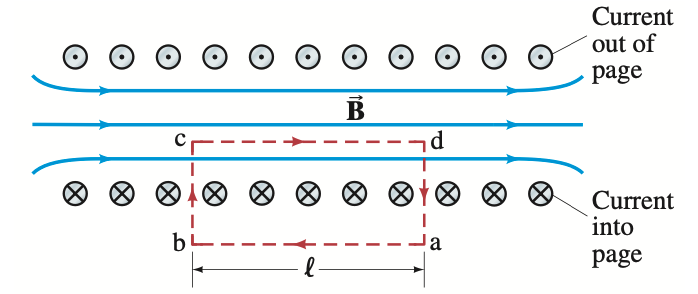
\includegraphics[scale = 0.3]{Images/Magnetisme/SpoelMagnetischVeld}
    \end{center}

    We berkenen nu de formule van het magnetisch veld van een spoel:
    \begin{align*}
        \oint \Vec{B} \cdot d\Vec{\ell} &= \mu_{0}NI \\
        B\ell &=  \mu_{0}NI \\
        B &=  \mu_{0}nI
    \end{align*}
    met $n= \tfrac{N}{\ell}$ het aantal windingen per lengte.
\end{theo}

\newpage

\begin{app}[Magnetisch veld van een torus]{Magnetisch veld van een torus}
    \begin{minipage}{.73\textwidth}
        We kunnen de wet van Ampère gebruiken om het magnetisch veld in de torus en buiten de torus te berekenen.
        \begin{enumerate}
            \item \textbf{Binnen de torus:} als we de wet van Ampère toepassen op pad 1 vinden we 
            \begin{align*}
                \oint \Vec{B} \cdot d\Vec{\ell} &= \mu_{0}I_{\text{encl}} \\
                        B(2 \pi r) &= \mu_{0}NI
            \end{align*}
            waarbij $N$ de hoeveelheid windingen en $I$ de stroom in deze windingen.
            % \item \textbf{Buiten de torus:}
        \end{enumerate}
    \end{minipage}
    \begin{minipage}{.23\textwidth}
        \vspace{-0.55cm}
        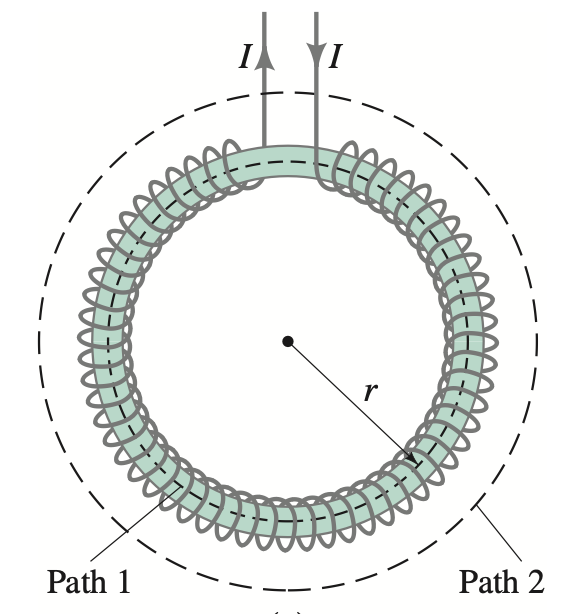
\includegraphics[scale = 0.4]{Images/Magnetisme/MagnetischVeldTorus.png}
    \end{minipage}
    \begin{enumerate}
        \setcounter{enumi}{1}
        \item \textbf{Buiten de torus:} het pad buiten de torus bevat $N$ windingen die stroom $I$ in één richting bevat en $N$ windingen
        die stroom $I$ in de tegengestelde bevat. Hierdoor wordt de ingesloten stroom $I_{\text{encl}} = 0$ en volgt dus
        \begin{align*}
            \oint \Vec{B} \cdot d\Vec{\ell} &= \mu_{0}I_{\text{encl}} \\
                    B(2 \pi r) &= 0
        \end{align*}
        en dus
        \begin{equation*}
            B = 0
        \end{equation*}
    \end{enumerate}
\end{app}

\begin{lem}[Biot-savart]{Biot-savart}
    Een stroom die vloeit door een bepaald pad kan bekeken worden door vele, infinitesimale
    stroomelementen
    % , in formulevorm:
    % \begin{equation*}
    %     I = \int I d\Vec{\ell}.
    % \end{equation*}
    Als $d\Vec{\ell}$ een infinitesimale lengte voorstelt waardoor stroom
    vloeit, dan is het magnetisch veld $d\Vec{B}$, op eenderwelk punt $P$ in de ruimte, door
    dit stroomelement gegeven door
    \begin{align*}
        d\Vec{B} &= \dfrac{\mu_{0}I}{4\pi}\dfrac{d\Vec{\ell} \times \hat{r}}{r^2} \\
              dB &= \dfrac{\mu_{0}I}{4\pi}\dfrac{d\ell}{r^2}\sin{(\theta)}
    \end{align*}
    waarbij $\Vec{r}$ de verplaatsingsvector is van het element $d\Vec{\ell}$ tot het punt $P$.
    We zien dus nu dat 
    \begin{itemize}
        \item de veldsterkte minimaal is, als $\forall k \in \mathbb{N}^{+}: \ \theta = 0^{\circ} + k(180^{\circ})$
        \item de veldsterkte maximaal is, als $\forall k \in \mathbb{N}^{+}: \theta = 90^{\circ} + k(180^{\circ})$
    \end{itemize} 
    Het totale magnetische veld in punt P vinden we dan door de integraal te nemen over alle stroomelementen
    \begin{equation*}
        \Vec{B} = \int d\Vec{B} = \dfrac{\mu_{0}I}{4\pi} \int \dfrac{d\Vec{l} \times \hat{r}}{r^{2}}
    \end{equation*}
    % Een belangrijk onderscheid tussen de wet van Biot-Savart en de wet van Ampère is dat bij de wet van Ampère
    % het magnetisch veld $\Vec{B}$ niet noodzakelijk enkel door de stroom is bij het integratiepad. Maar bij de wet
    % van Biot-Savart is het magnetisch veld $d\Vec{B}$ enkel en volledig bepaald door het stroomelement $Id\Vec{\ell}$.
    % Om het totale magnetisch veld $\Vec{B}$ te vinden is het noodzakelijk om de alle stroom te includeren.
    Deze wet is vooral nuttig als we geen symmetrie kunnen gebruiken, en dus niet de wet van Ampère kunnen gebruiken.
\end{lem}

% \begin{vrg}[Verschil tussen de wet van Ampère en de wet van Biot-Savart]{Verschil tussen de wet van Ampère en de wet van Biot-Savart}
%     Een belangrijk onderscheid tussen de wet van Biot-Savart en de wet van Ampère is dat bij de wet van Ampère
%     het magnetisch veld $\Vec{B}$ niet noodzakelijk enkel door de stroom is bij het integratiepad. Maar bij de wet
%     van Biot-Savart is het magnetisch veld $d\Vec{B}$ enkel en volledig bepaald door het stroomelement.
%     Om het totale magnetisch veld $\Vec{B}$ te vinden is het noodzakelijk om de alle stroom te includeren.
% \end{vrg}

\newpage

% \begin{theo}[Magnetisme in materialen]{Magnetisme in materialen}
    
% \end{theo}

